%%%%%%%%%%%%%%%%%%%%%%%%%%%%%%%%%%%%%%%%%
% Jacobs Landscape Poster
% LaTeX Template
% Version 1.1 (14/06/14)
%
% Created by:
% Computational Physics and Biophysics Group, Jacobs University
% https://teamwork.jacobs-university.de:8443/confluence/display/CoPandBiG/LaTeX+Poster
% 
% Further modified by:
% Nathaniel Johnston (nathaniel@njohnston.ca)
%
% This template has been downloaded from:
% http://www.LaTeXTemplates.com
%
% License:
% CC BY-NC-SA 3.0 (http://creativecommons.org/licenses/by-nc-sa/3.0/)
%
%%%%%%%%%%%%%%%%%%%%%%%%%%%%%%%%%%%%%%%%%

%----------------------------------------------------------------------------------------
%	PACKAGES AND OTHER DOCUMENT CONFIGURATIONS
%----------------------------------------------------------------------------------------

\documentclass[final]{beamer}

\usepackage[scale=1.14]{beamerposter} % Use the beamerposter package for laying out the poster

\usetheme{confposter} % Use the confposter theme supplied with this template

\setbeamercolor{block title}{fg=ngreen,bg=white} % Colors of the block titles
\setbeamercolor{block body}{fg=black,bg=white} % Colors of the body of blocks
\setbeamercolor{block alerted title}{fg=white,bg=dblue!70} % Colors of the highlighted block titles
\setbeamercolor{block alerted body}{fg=black,bg=dblue!10} % Colors of the body of highlighted blocks
% Many more colors are available for use in beamerthemeconfposter.sty

%-----------------------------------------------------------
% Define the column widths and overall poster size
% To set effective sepwid, onecolwid and twocolwid values, first choose how many columns you want and how much separation you want between columns
% In this template, the separation width chosen is 0.024 of the paper width and a 4-column layout
% onecolwid should therefore be (1-(# of columns+1)*sepwid)/# of columns e.g. (1-(4+1)*0.024)/4 = 0.22
% Set twocolwid to be (2*onecolwid)+sepwid = 0.464
% Set threecolwid to be (3*onecolwid)+2*sepwid = 0.708

\newlength{\sepwid}
\newlength{\onecolwid}
\newlength{\twocolwid}
\newlength{\threecolwid}
\setlength{\paperwidth}{46.8in} % A0 width: 46.8in
\setlength{\paperheight}{40in} % A0 height: 33.1in
\setlength{\sepwid}{0.012\paperwidth} % Separation width (white space) between columns
\setlength{\onecolwid}{0.22\paperwidth} % Width of one column
\setlength{\twocolwid}{0.464\paperwidth} % Width of two columns
\setlength{\threecolwid}{0.708\paperwidth} % Width of three columns
\setlength{\topmargin}{-0.5in} % Reduce the top margin size
%-----------------------------------------------------------

\usepackage{graphicx}  % Required for including images

\usepackage{booktabs} % Top and bottom rules for tables

%----------------------------------------------------------------------------------------
%	TITLE SECTION 
%----------------------------------------------------------------------------------------

\title{A Monte-Carlo based approach for estimating \\remote sensing reflectance uncertainty} % Poster title

\author{Erdem M. Karak\"{o}yl\"{u}$^{1,2}$ \and Bryan Franz$^{1}$} % Author(s)
\institute{1: Science Applications International Corporation \\
           2: Ocean Biology Processing Group - NASA Goddard Space Flight Center} % Institution(s)

%----------------------------------------------------------------------------------------

\begin{document}

\addtobeamertemplate{block end}{}{\vspace*{2ex}} % White space under blocks
\addtobeamertemplate{block alerted end}{}{\vspace*{2ex}} % White space under highlighted (alert) blocks

\setlength{\belowcaptionskip}{2ex} % White space under figures
\setlength\belowdisplayshortskip{2ex} % White space under equations

\begin{frame}[t] % The whole poster is enclosed in one beamer frame

\begin{columns}[t] % The whole poster consists of three major columns, the second of which is split into two columns twice - the [t] option aligns each column's content to the top

\begin{column}{\sepwid}\end{column} % Empty spacer column

\begin{column}{\onecolwid} % The first column

%----------------------------------------------------------------------------------------
%	OBJECTIVES
%----------------------------------------------------------------------------------------

\begin{alertblock}{Objectives}

\begin{itemize}
\item Implement self-contained sensor-dependent (SeaWiFS showcased) noise model.
\item Characterize noise propagation due to atmospheric correction.
\item Characterize impact of noise in near-infrared bands
\item Generate remote sensing reflectance uncertainty product.
\end{itemize}

\end{alertblock}

%----------------------------------------------------------------------------------------
%	INTRODUCTION
%----------------------------------------------------------------------------------------

%\begin{block}{Introduction}


%\begin{itemize}
%\item Ocean color missions subject to pre-specified uncertainty requirements.
%\item Uncertainty difficult to estimate consistently
%\item Typical uncertainty estimation done using potentially problematic comparisons\cite{BW:2006,Tle:2000,Hu:2013}	 
%\end{itemize}
%\end{block}


%----------------------------------------------------------------------------------------
%	METHODS - ditch that change to Approach
%----------------------------------------------------------------------------------------

\begin{block}{Methods}
\begin{itemize}
\item Model signal-to-noise Ratio (SNR) as a function of $L_t$\cite{Barnes:1994} .
\item Spread in noise distribution given by $\sigma = \frac{L_t}{SNR}$.
\item $L_{t,NOISE} = N(L_t, \sigma^2)$
\item Propagate noise through atmospheric correction, retrieve remote sensing reflectance ($Rrs$).
\item Use steps above to run Monte-Carlo Simulation.
\end{itemize}
\end{block}
\begin{figure}
\centering
\textbf{Signal-to-noise ratio as a function of top-of-the-atmosphere radiance ($L_t$)}\par\medskip
%
\includegraphics[width=1.0\linewidth]{placeholder.jpg}
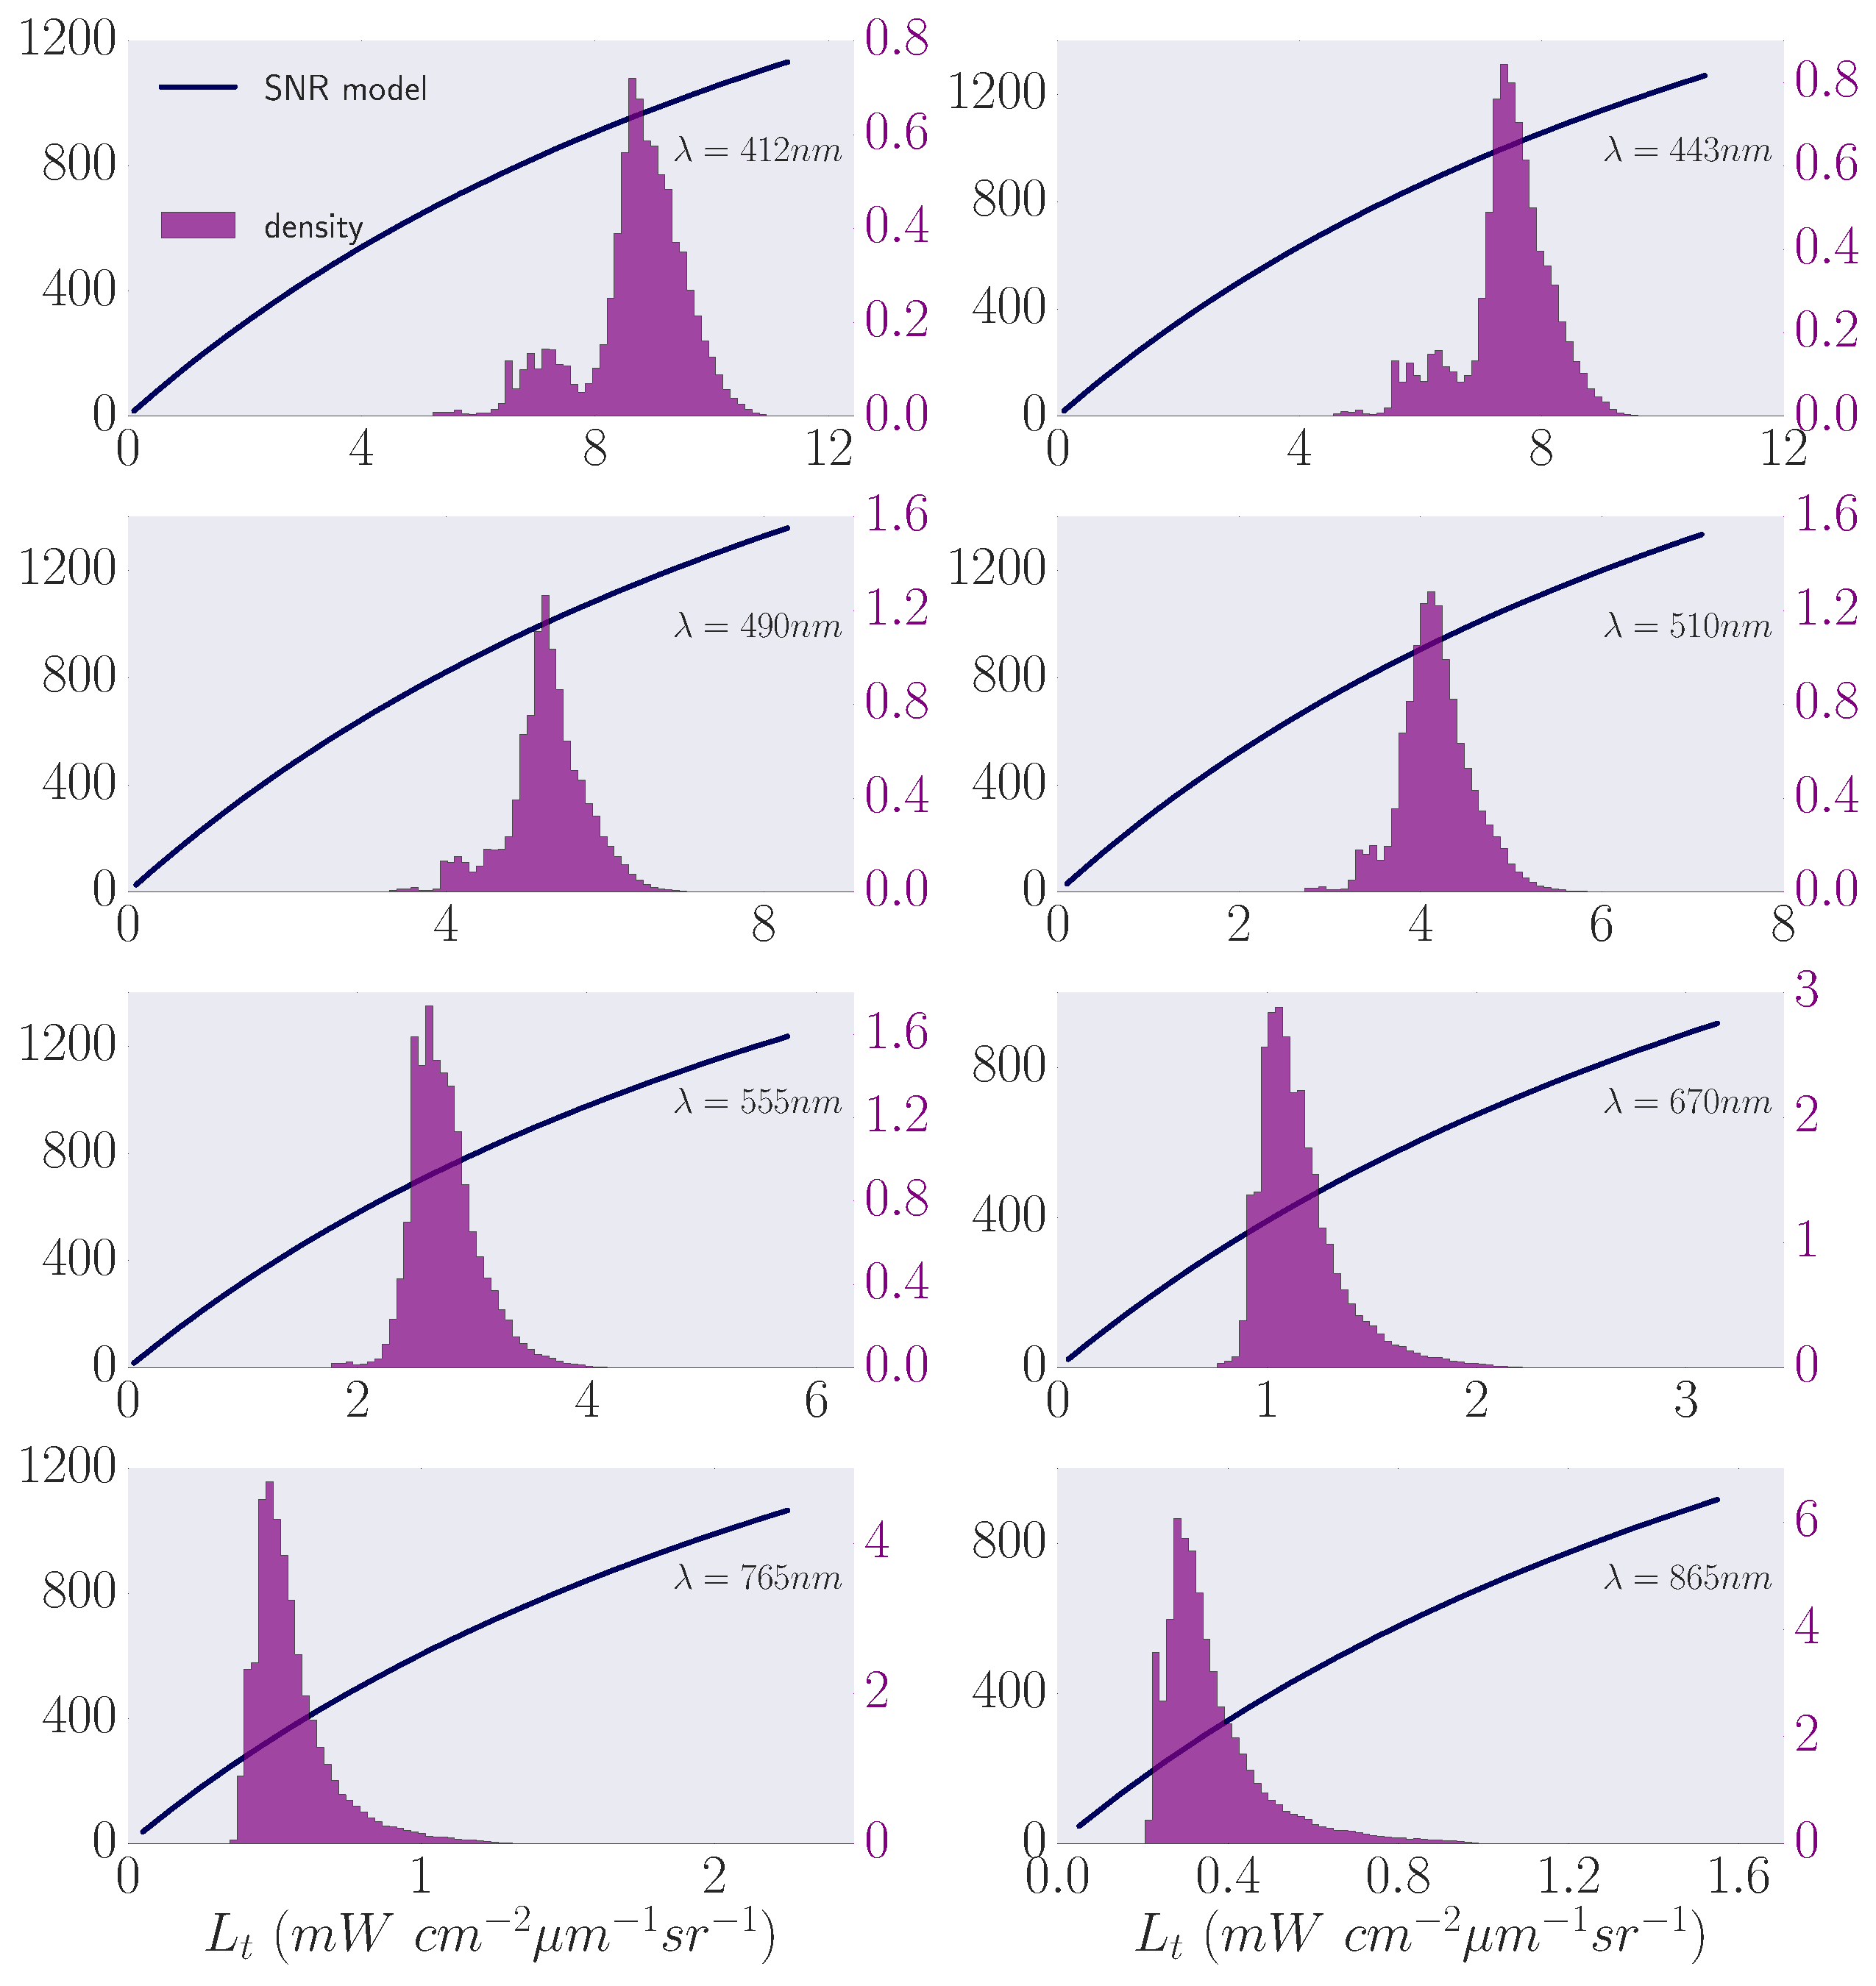
\includegraphics[width=1.0\linewidth]{snrmodelLong.pdf}
\end{figure}

% Add sensitivity analysis after this, just one of the plots.




%----------------------------------------------------------------------------------------

\end{column} % End of the first column

\begin{column}{\sepwid}\end{column} % Empty spacer column

\begin{column}{\twocolwid} % Begin a column which is two columns wide (column 2)
%----------------------------------------------------------------------------------------
%	RESULTS - remove sensitivity analysis figures here, 
%  Do some side by side comparisons of distributions of 
%  Rrs_unc for 
%----------------------------------------------------------------------------------------
\begin{block}{Results}

\begin{columns}[t,totalwidth=\twocolwid] % Split up the two columns wide column

\begin{column}{\onecolwid}\vspace{-.6in} % The first column within column 2 (column 2.1)

\begin{figure}
%
\includegraphics[width=1.0\linewidth]{placeholder.jpg}
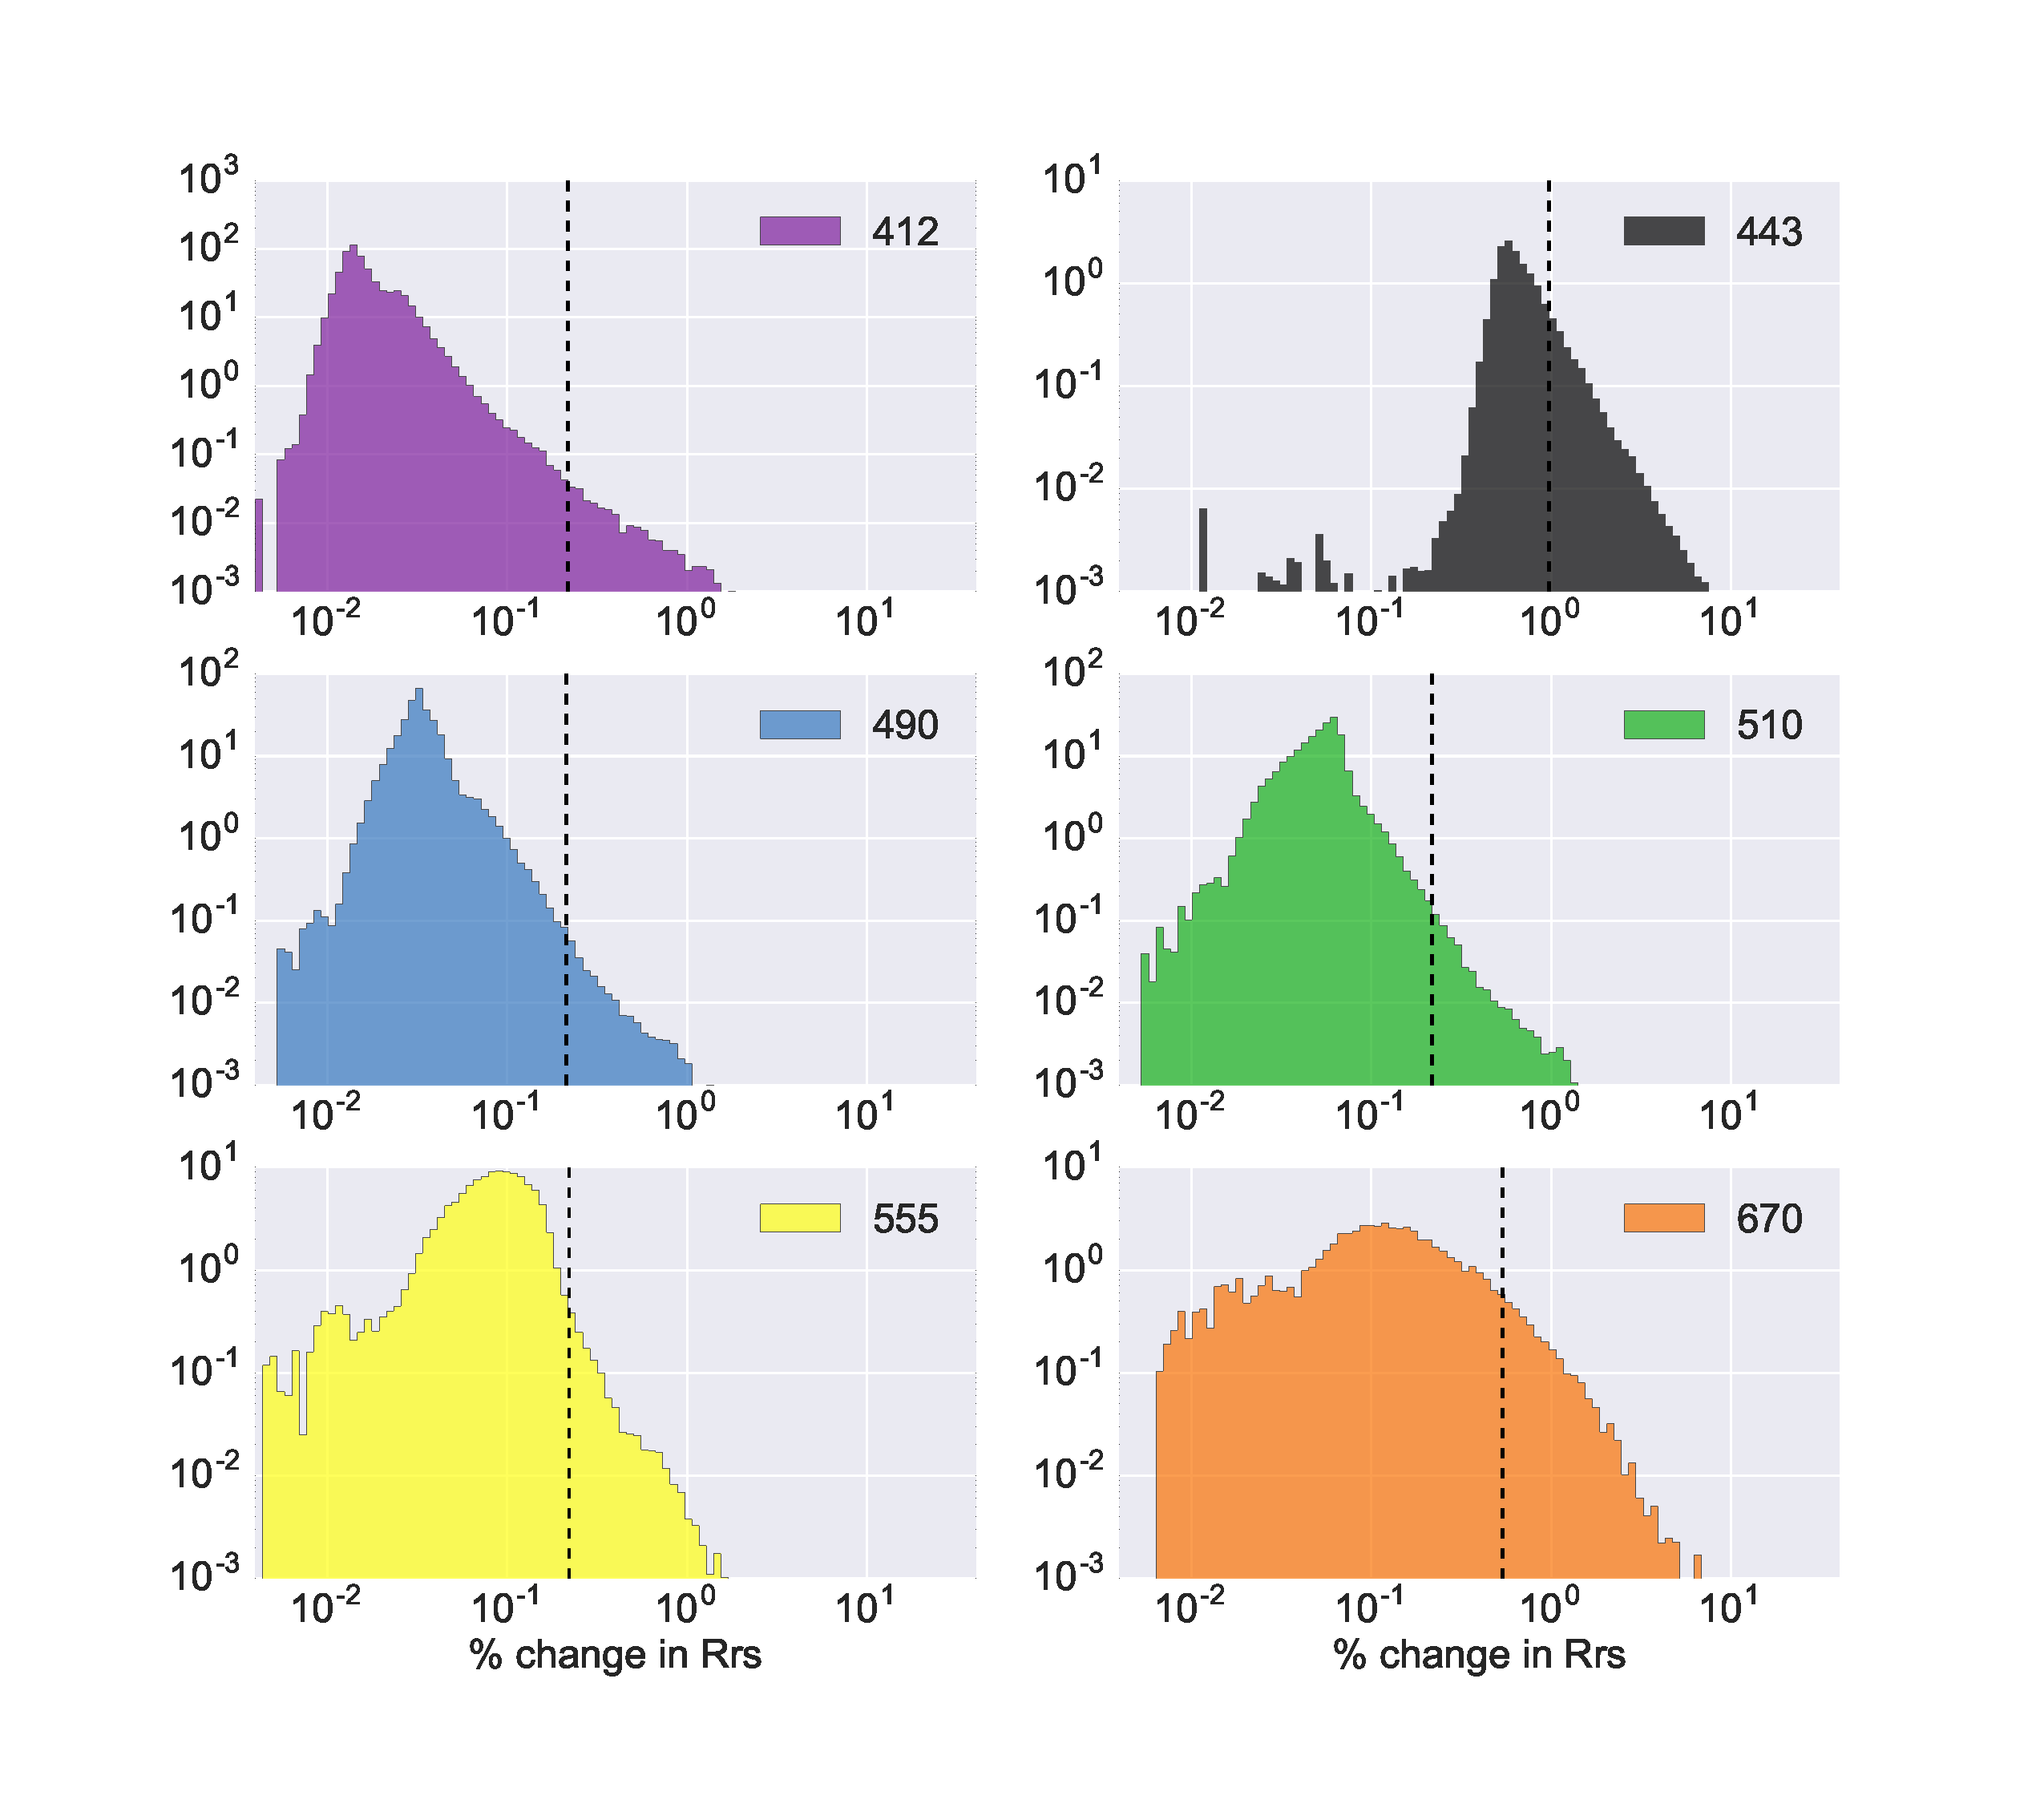
\includegraphics[width=1.1\linewidth]{Propagation443.pdf}
\\{Figure caption}
\end{figure}


\end{column} % End of column 2.1

\begin{column}{\onecolwid}\vspace{-.6in} % The second column within column 2 (column 2.2)


\begin{figure}
%
\includegraphics[width=1.0\linewidth]{placeholder.jpg}
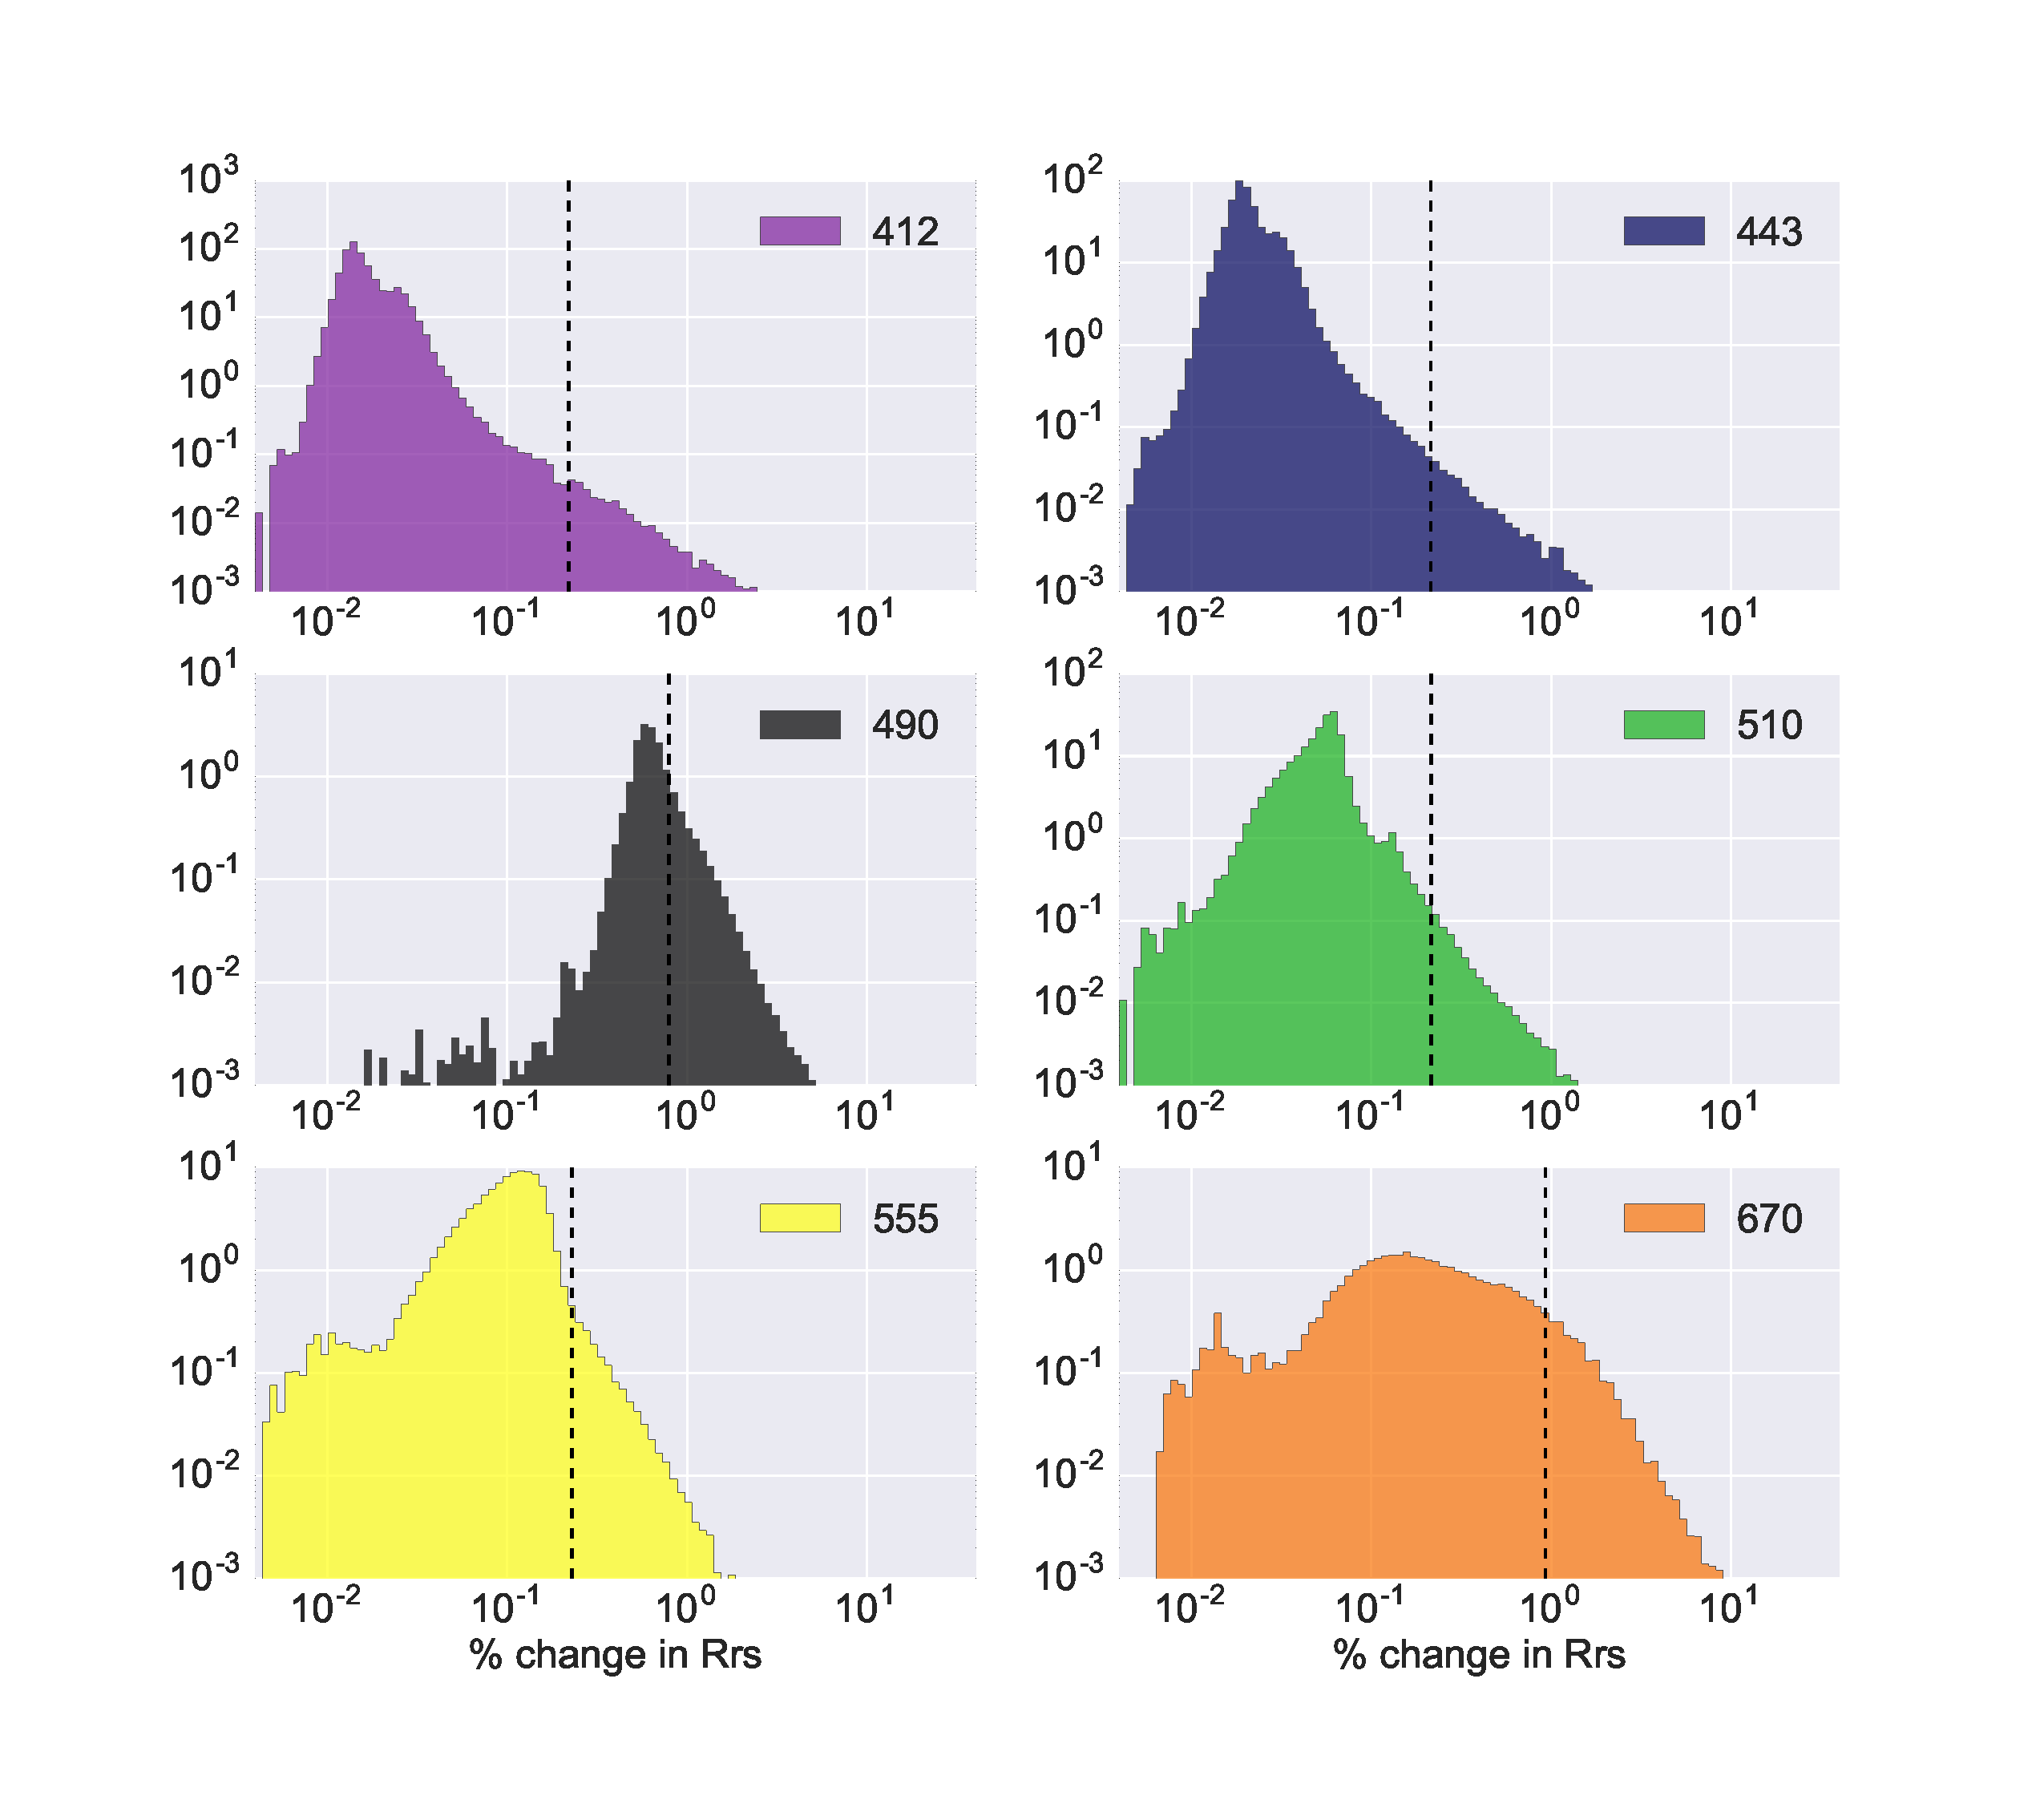
\includegraphics[width=1.1\linewidth]{Propagation490.pdf}
\\{Figure caption}
\end{figure}

\begin{figure}
\centering
\textbf{My Title}\par\medskip

\includegraphics[width=0.8\linewidth]{placeholder.jpg}
\\{Figure Caption}
\end{figure}

\end{column} % End of column 2.2

\end{columns} % End of the split of column 2 - any content after this will now take up 2 columns width
\end{block}
\begin{figure}
\centering
\textbf{Global1}\par\medskip
\includegraphics[width=1.0\linewidth]{global412.png}
\\{Nunc tempus venenatis facilisis. Curabitur suscipit consequat eros non porttitor. Sed a massa dolor, id ornare enim}
\end{figure}

\begin{columns}[t,totalwidth=\twocolwid] % Split up the two columns wide column again
\begin{column}{\onecolwid} % The first column within column 2 (column 2.1)






%----------------------------------------------------------------------------------------

\end{column} % End of column 2.2

\end{columns} % End of the split of column 2

\end{column} % End of the second column

\begin{column}{\sepwid}\end{column} % Empty spacer column

\begin{column}{\onecolwid} % The third column

%----------------------------------------------------------------------------------------
%	What's next?
%----------------------------------------------------------------------------------------

\begin{block}{Next Steps}
\begin{itemize}
\item Extend MC simulations to other sensors.
\item MC simulations computationally costly;
	\begin{itemize}
	\item Finding an alternative to build on this work, a priority
	\item Develop machine learning (ML) approach (e.g. neural network);
	\item Identify uncertainty drivers in MC as potential inputs to ML;
 	\item Use ML to shorten uncertainty product generation to one run. 
	\end{itemize}
\end{itemize}

\end{block}


%----------------------------------------------------------------------------------------
%	REFERENCES
%----------------------------------------------------------------------------------------

\begin{block}{References}
\nocite{} % Insert publications even if they are not cited in the poster
\small{\bibliographystyle{IEEEtran}
\bibliography{poster}\vspace{0.75in}}

\end{block}

%----------------------------------------------------------------------------------------
%	ACKNOWLEDGEMENTS
%----------------------------------------------------------------------------------------

\setbeamercolor{block title}{fg=red,bg=white} % Change the block title color

\begin{block}{Acknowledgements}

\small{\rmfamily{We thank \textit{Don Shea} and \textit{Sean Bailey} for assistance with l2gen integration of the MC code, and to \textit{Tommy Owens} for running large scale MC simulations on the OBPG production system.}} \\

\end{block}

%----------------------------------------------------------------------------------------
%	CONTACT INFORMATION
%----------------------------------------------------------------------------------------

\setbeamercolor{block alerted title}{fg=black,bg=norange} % Change the alert block title colors
\setbeamercolor{block alerted body}{fg=black,bg=white} % Change the alert block body colors

\begin{alertblock}{Contact Information}

\begin{itemize}
\item Web: \href{oceancolor.gsfc.nasa.gov}{oceancolor.gsfc.nasa.gov}
\item Email: \href{mailto:erdem.m.karakoylu@nasa.gov}{erdem.m.karakoylu@nasa.gov}
\item Phone: +1 (301) 286 0501
\end{itemize}

\end{alertblock}

\begin{center}
\begin{tabular}{ccc}

\includegraphics[width=0.4\linewidth]{NASA_logo.png} & \hfill 
\end{tabular}
\end{center}

%----------------------------------------------------------------------------------------

\end{column} % End of the third column

\end{columns} % End of all the columns in the poster

\end{frame} % End of the enclosing frame

\end{document}
